\section{Related Work}
\subsection{Matrix Factorization}
In this section, I review some existing work on recommendation system with matrix factorization techniques, integrating social trust. Firstly, matrix factorization has been one of most popular approaches in the domain of collaborative filtering, which is traditionally one of the typical methods for recommendation system. In collaborative filtering, there are a set of $m$ users $\mathcal{U} = \{U_1,U_2,...,U_m\}$ and a set of $n$ items $\mathcal{V} = \{V_1,V_2,...,V_n\}$, where each user $u_i$ may express their preference to some items by giving a rating in a range. For example, in Netflix, users will rate the movies from 1 to 5 star they watched to show how much they like the movie. Therefore, the rating matrix $R \in \mathbb{R}^{m \times n}$ is formed, in which the rows and columns represent the users and items, respectively. And an entry in $R_{ij}$ records the rating user $U_i$ gave to the item $V_j$. 

In reality, most of the entries in the rating matrix R are unknown because one user only rates a small number of items, making the matrix very sparse. We need to predict the missing rating a user gives to an item based on his or her history ratings. Matrix Factorization technique, one of the most popular approaches, is based on the assumption that there are a small number of latent factors deciding the items' properties and users' preferences. Then the rating $R_{ij}$ user $U_i$ give to the item $V_j$ can be predicted by the inner product of two latent feature vectors, which is shown in equation (5). Further, the model is trained on the observed rating data by minimizing the square error(with the usual Frobenius/L2-norm regularization), which is the equation (3) and (4)(see also \cite{koren2009matrix}).

In \cite{mnih2007probabilistic}, the author gives a probabilistic explaination to the matrix factorization. They adopt a probabilistic linear model with Gaussian observation noise(see fig.1), and define the conditional distribution over the observed ratings as
\begin{equation}
p(R|U,V,\sigma^2) = \prod_{i=1}^{M}\prod_{j=1}^{N}\big[\mathcal{N}(R_{ij}|U_i^TV_j,\sigma^2)\big]^{I_{ij}},
\end{equation} 
where $\mathcal{N}(R_{ij}|U_i^TV_j,\sigma^2)$ is a probability density function of the Gaussian distribution with mean $\mu$ and variance $\sigma^2$, and $I_{ij}$ is the indicator function that is equal to 1 if user i rated item j and equal to 0 otherwise. Zero-mean spherical Gaussian priors are also placed on user and item feature vectors, 
\begin{equation}
p(U|\sigma_U^2) = \prod_{i=1}^{M}\mathcal{N}(U_{i}|0,\sigma_U^2\bold{I}),\quad\quad
p(V|\sigma_V^2) = \prod_{j=1}^{N}\mathcal{N}(V_{j}|0,\sigma_V^2\bold{I}),
\end{equation} 
Then by maximizing the log of posterior distribution over the user and movie features,
\begin{equation}
ln(p(U,V|R, \sigma^2,\sigma_U^2,\sigma_V^2)) = -\frac{1}{2\sigma^2}\sum_{i=1}^{M}\sum_{j=1}^{N}I_{ij}(R_{ij} - U_i^TV_j)^2 - \frac{1}{2\sigma_U^2}\sum_{i=1}^{M}U_i^TU_i - \frac{1}{2\sigma_V^2}\sum_{j=1}^{N}V_j^TV_j + C,
\end{equation} 
( where C is a constant that does not depend on the parameters) is equivalent to minimizing the sum-of-squared-erros objective function with quadratic regularization terms:
\begin{equation}
\min_{U,V}\frac{1}{2}\sum_{i=1}^{M}\sum_{j=1}^{N}I_{ij}(R_{ij} - U_i^TV_j)^2 + \frac{\lambda_1}{2}||U||_F^2 + \frac{\lambda_2}{2}||V||_F^2,
\end{equation} 
\begin{figure}[h]
	\caption{i)the left one is the graphical representation of Probabilistic Matrix Factorization (PMF); ii)the right one is the graphical representation of SoRec.}
	\centering
	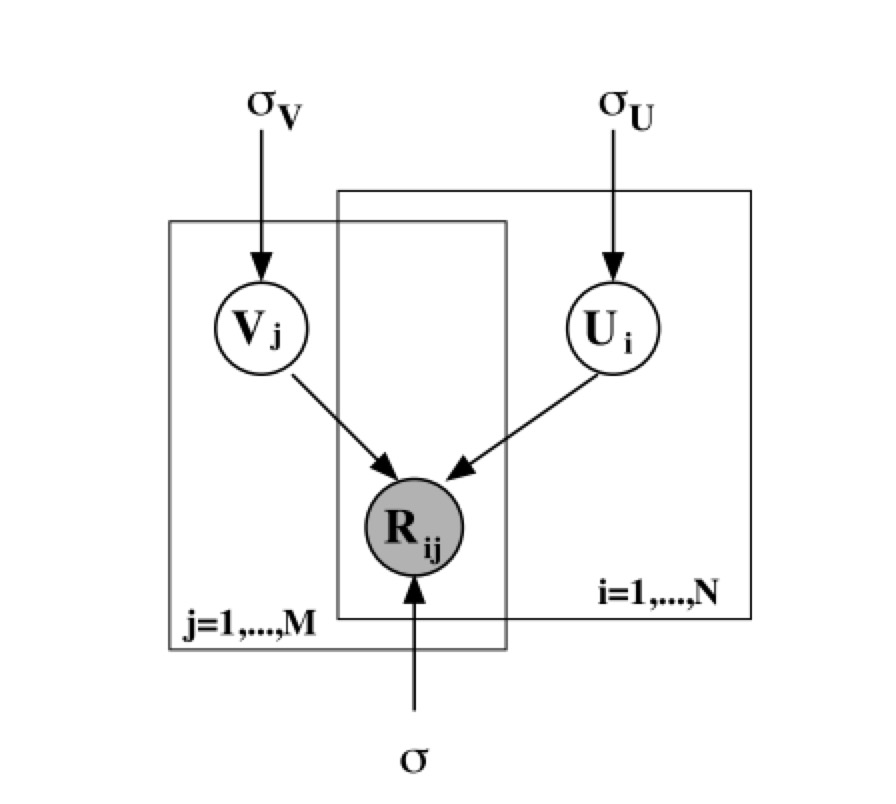
\includegraphics[width=8cm]{pmf}
	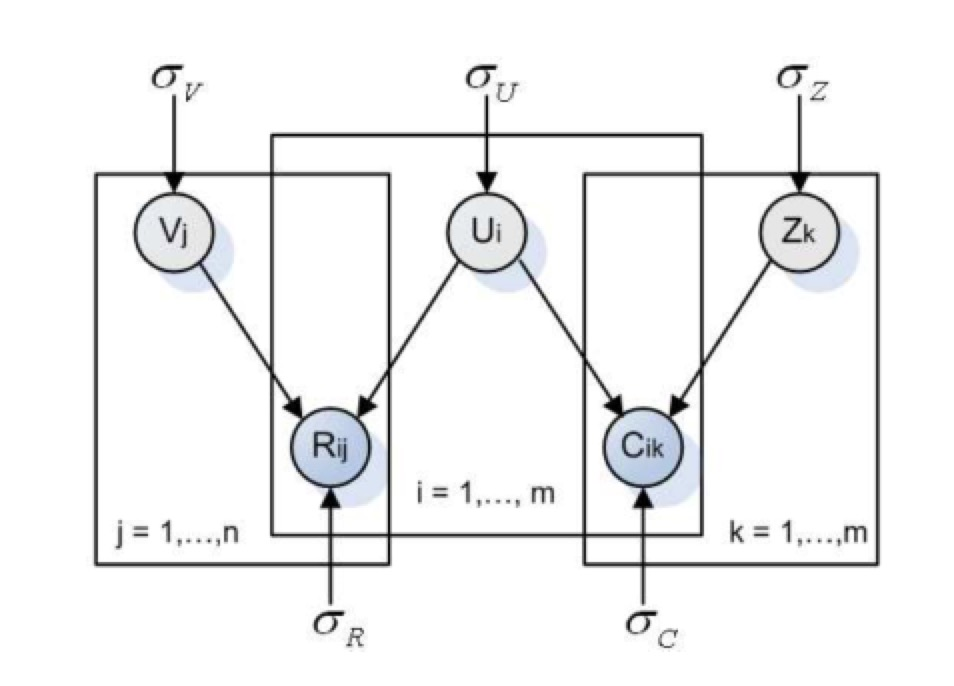
\includegraphics[width=8cm]{sorec}
\end{figure}

\textcolor{red}{\textbf{advantage and disadvantage of related work should be elaborated explicitly.}}

\subsection{Matrix Factorization with social networks and trust}
MF and PMF have been the most popular techniques for rating prediction. However, there are two main problems facing them:cold start and sparsity. Cold start refers to that new users or items that do not have any ratings. And sparsity refers to the fact that the matrix is sparse. To address these two problems, researchers tried to integrate different side information into the matrix factorization framework, among which the social factors stand out because the booming of online social networks during recent years. \cite{jamali2010matrix}\cite{ma2009llearningEnsembel}\cite{ma2009learningTrust}\cite{ma2008sorec}\cite{ma2011recommender}\cite{massa2004trust}\cite{yang2013social}. The underlying assumption of all the work is that users can affect and be affected by his friends when rating an item, while in the standard MF, all the users and items are considered independent and identically distributed(i.i.d).

Apart from the rating matrix $R$, there is one more matrix $S^{m \times m}$ representing the social network with m nodes, where the nodes represent users and the arcs represent connections between users. $S_{ij}$ is a real value describing the strength of connection between user $U_i$ and $U_j$. In \cite{ma2008sorec}, the SoRec model is proposed to integrate the social network into the probabilistic matrix factorization framework. The two matrices are connected by an assumption that the user latent feature space in the social network matrix is the same in the user\_item rating matrix.(see figure 1). By co-factorizing the rating and social matrix, the low-rank user-specific and item-specific latent features are learned by a similar gradient descent method. There is another underlying assumption that an user's rating are affected by his or her friends in the social networks. The experimental analysis shows the method generates better recommendations than the traditional collaborative filtering algorithms. However, the disadvantage of this work is that it lacks physical interpretations, which does not reflect the real world recommendation process.

Then in \cite{ma2009llearningEnsembel} and \cite{ma2009learningTrust}, Ma et al. further explore how the connections between users affect their rating behaviors. Based on a very intuitive assumption that an user's preferences is closer to the people he or she trusts or likes but farther to those he or she distrusts or dislikes. In \cite{ma2009llearningEnsembel}, the authors interpret one user's final ratings as the balance between this user's own taste and his or her trusted users' favors. Finally, an ensemble probabilistic matrix factorization method is proposed to model this process. The experimental results demonstrate that this approach can better model the problem. In \cite{ma2009learningTrust}, the authors try to incorporate the trust and distrust relations respectively into the rating process. They make the trust and distrust information as regularization terms to the MF objective functions and then perform a similar gradient descent method to calculate the user-specific and item-specific latent features. Their experiments also show the improving performance of prediction while an obvious problem facing this method, which is that they just treat distrust the same way as trust. However, in reality, distrust affects people's decision not the same way as trust does. Besides, trust and distrust are regularized respectively thus a very straightforward improved direction is to fuse these two data sources into the same objective function. 

In \cite{jamali2010matrix}, the author extent the work of \cite{ma2009llearningEnsembel} by taking into account trust propagation, which is not considered previously. The model is proposed according to the theory from social influence that the behavior of a user $u$ is affected by his direct neighbors $N_u$. In specific speaking, the latent feature vector of $u$ is dependent on the latent feature vector of all his direct neighbors $v \in N_u$. Then the influence is formulated as 
\begin{equation}
\widehat{U}_u = \frac{\sum_{v \in N_u} T_{u,v}U_u}{\sum_{v \in U_u}T_{u,v}} = \frac{\sum_{v \in N_u} T_{u,v}U_u}{|N_u|},
\end{equation}
where $\widehat{U}_u$ is the estimated latent feature vector of $u$ given the feature vectors of his direct neighbors. Recursively, the latent feature vector of each direct neighbor is dependent on the feature vector of his direct neighbors, leading to the propagation of trust. Finally, a very similar objective function to that in \cite{ma2009learningTrust} is given and it is calculated by the gradient descend method too. The performance is also improved in two real datasets, which demonstrates the effectiveness of the exploition of trust propagation. An potential improving direction of this work is to handle distrust relations, whose propagation is surely different from trust.

So far, three general techniques are employed to incorporate the social factors: co-factorization \cite{ma2008sorec} and regularization \cite{ma2009learningTrust}\cite{jamali2010matrix} and ensemble method\cite{ma2009llearningEnsembel}. Actually, the following work of this direction are mostly utilizing these three techniques. In \cite{ma2011recommender}, Ma et al. systematically illustrate how to design a matrix factorization objective function with social regularization, which can also be easily extended to incorporate other side information like contextual information, social tags, etc. Two regularization terms are proposed in this work. One is average-based, whose underlying assumption is that every user's taste is close to the average taste of this user's friends. The other one is individual-based, which requires that the more similar two users are, the closer their latent features should be. The advantage of this work is not only improving the performance of recommendation, but also give a general way to incorporate side information to MF framework. All of the following work \cite{Forsati:2015:PER:2792838.2800198} \cite{li2015overlapping} \cite{yang2013social} use a similar regularization method to incorporate other side information into the MF framework and improve the performance.

In summary, all the aforementioned approaches are regarding the social or trust relations as side information to address the cold start and sparsity. And experiments in real datasets demonstrate the effectiveness of these methods. One underlying assumption all the methods share is that one user will be affected by his/her friends in social network or trust people in all aspects. However, this is no always true. In \cite{yang2012circle}, X. Yang et al. argue that a user may trust different subsets of friends regrading different domains. For example, we may ask some friends for recommendations when buying cars while others when buying cellphones. In other words, the trust is domain- or category- specific. Therefore, the authors propose a circle-based matrix factorization framework, which tries to infer category\-specific social trust circles from the rating data combined with social network data where social trust links across all categories are mixed together. However, the method need to utilize the category information of items while in most cases they are not accessible. Therefore, an category inferring approaches are proposed in this paper, which tries to learn the implicit domain-specific trust.

